\chapter{Testes e Avaliação do Jogo}

\label{cap5}

\todo{Analisar}

Com o objetivo de analisar o projeto desenvolvido, foram aplicados dois formulários: um antes da sessão de jogo e outro após a sua conclusão. O objetivo destes formulários consiste em avaliar se existe um aumento dos conhecimentos dos participantes após a experiência de jogo. O objetivo do jogador durante o teste é chegar até ao 1º ataque de \textit{DDos}.

Em simultâneo, as sessões de jogo de cada participante foram analisadas com o objetivo de identificar padrões de utilização e oportunidades de melhoria ao nível da \ac{UX}. Os dados recolhidos durante estas sessões foram analisados com base nas heurísticas de usabilidade propostas por \textcite{nielsen1994enhancing}, cuja aplicação será detalhada nas subsecções seguintes.

A escolha destas heurísticas como métrica de avaliação deve-se à natureza dos dados em análise, uma vez que estas foram desenvolvidas especificamente para avaliar a experiência do utilizador.

Para além das métricas anteriormente referidas, foram ainda recolhidos dados de telemetria de forma automática durante cada sessão de jogo. Para esse efeito, foi utilizada a plataforma \textbf{Firebase} para armazenar essa informação. O objetivo desta recolha consiste em identificar padrões relacionados com os tempos de interação dos jogadores em diferentes situações, permitindo perceber se existem momentos da \textit{gameplay} que apresentam comportamentos significativamente discrepantes relativamente aos restantes.

\section{Analise qualitativa da \ac{UX}}

\begin{table}[H]
    \centering
    \begin{tabular}{|p{4.5cm}|c|p{3cm}|p{4.5cm}|}
        \hline
        \textbf{Problema} & \textbf{Grau} & \textbf{Heuristica} & \textbf{Solução} \\ \hline
        Falta de \textit{feedback} no sistema de som & Baixo & Visibilidade do estado do sistema & Adição uma \textit{label} informativa \\ \hline
        Falta de \textit{feedback} nos botões de notificações & Média & Visibilidade do estado do sistema & Adição de instruções mais claras ao lado dos botões \\ \hline
        Controlos do canhão & Elevado & Controlos do utilizador e liberdade / Consitência e padronização & Inverter os commandos \\ \hline
        Jogador não se lembra como abrir a loja & Elevado & Reconhecimento em vez de memorização & Adição de indicativo visual na \ac{UI}. \\ \hline
        Jogador não têm noção da finalidade dos componentes de \textit{hardware} & Elevado & Correspondência entre o sistema e o mundo & Adição de uma label com uma pequena descrição do componente na loja \\ \hline
        Falta de \textit{feedback} na configuração de um \ac{CPU} na tela da loja & Media & Visibilidade do estado do sistema & Adição de uma \textit{label} informativa. \\ \hline
        Falta de \textit{feedback} nos emails & Elevado & Visibilidade do estado do sistema & Adição de um idicador visual, que aparece sempre que existe um email por ler \\ \hline
        Câmara muito próxima do jogador & Baixo & Controlo e liberdade do jogador & Adição do controlo de zoom da câmara \\ \hline
    \end{tabular}
    \caption{Analise dos problemas usando as heuristicas de Nielsen}
    \label{tab:DadosNielsen}
\end{table}

Os dados recolhidos das observações das seções de jogo de dos jogadores que participaram nos testes encontrassam analisados
na tabela \ref{tab:DadosNielsen}.

\section{Analisa do conhecimento transmitido e das seções de jogo}

Esta seção é divida em várias sub seções, onde são analisados os dados recolhidos oriundos dos formulários assim como os dados de telemetria recolhidos ao logo de cada seção de jogo, tais como:
\begin{itemize}
    \item Tempo para comprar/configurar o 1º servidor;
    \item Tempo necessário para concluir cada mini game;
    \item Watts do servidores;
    \item Tempo que o jogador demorou para destruir o 1º ataque \textit{DDos};
    \item Tempo total da seção de jogo até a finalização do 1º ataque.
\end{itemize}

\subsection{Defenição da amostra}

A amostra utiliza para realizar um dado teste é facto primário que avalia a qualidade do mesmo, uma vez que se a amostra for muito pequena os resultados derivados dela podem não refletir a relidade de uma dada população (conjunto total de indivíduos ou objectos sobre os quais incide o estudo). Além do seu tamanho, uma boa amostra também deve ser diversas, uma vez que se uma amostra for pouco diversa ela irá gera viés estatísticos.

Posto isto a amostra recolhida para desenvolver os testes, é composta de um total de 25 individuos, de vários gêneros, e com uma faixa etária que varia desde [menos 18 anos até mais de 30 anos]. A seguir serão apresentados um conjunto de dados tabulares e em gráficos que a caracterização.

\begin{table}[H]
    \centering
    \begin{tabular}{|c|c|}
        \hline
        \textbf{Faixa de idades} & \textbf{Número de individuos} \\ \hline
        Menos de 18 anos & 2 \\ \hline
        18 a 24 anos & 10 \\ \hline
        25 a 29 anos & 11 \\ \hline
        30 a 34 anos & 2 \\ \hline
        Mais de 35 anos & 0 \\ \hline
    \end{tabular}
    \caption{Faixa de idades}
    \label{tab:Faixa_Idades}
\end{table}


A Tabela \ref{tab:Faixa_Idades} informa que maioria dos individuos se encontram entre os 18 e 29 anos, todavia, existe um pequeno conjunto que se encontra fora desse intrevalo.


\begin{table}[H]
    \centering
    \begin{tabular}{|c|c|}
        \hline
        \textbf{Conhecimentos em informática} & \textbf{Número de individuos} \\ \hline
        Possuir e tem formação académica na área da informática & 13 \\ \hline
        Apenas na ótica do utilizador & 4 \\ \hline
        Não possuir & 7 \\ \hline
    \end{tabular}
    \caption{Conhecimentos prévios em informática}
    \label{tab:Conhecemintos}
\end{table}

A partir da Tabela \ref{tab:Conhecemintos}, conclui-se que 52\% da amostra possui formação na área, enquanto os restantes 48\% não possuem qualquer formação ou possuem apenas formação na ótica do utilizador. Este dado é importante para interpretar o conhecimento prévio dos participantes, uma vez que os indivíduos que já possuem conhecimentos na área poderão não apresentar um incremento significativo.

\begin{figure}[H]
    \centering
    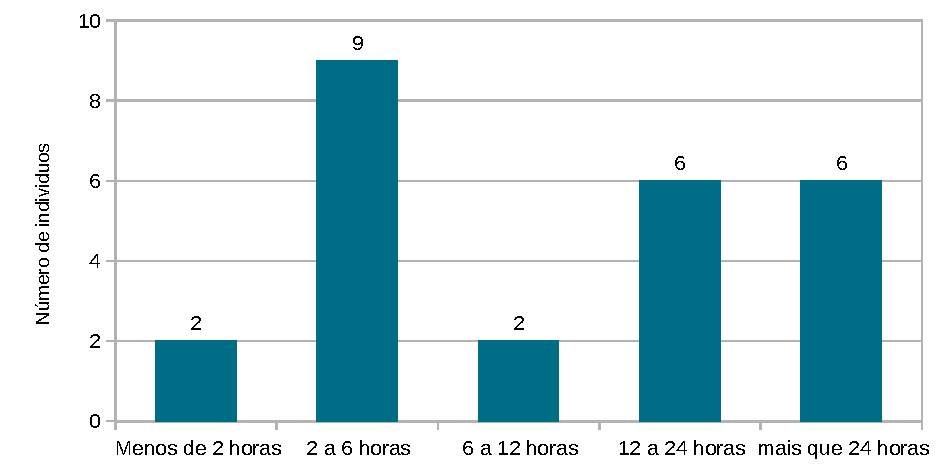
\includegraphics[width=0.8\textwidth]{images/Gráficos dos testes/Graficos de horas.pdf}
    \caption{Número de horas semanais dispensadas para jogar}
    \label{graph:Numero_Horas_Semanais}
\end{figure}

A partir do gráfico apresentado na Figura \ref{graph:Numero_Horas_Semanais}, verifica-se que a amostra é constituída por jogadores com diferentes níveis de horas. Esta variedade poderá influenciar os resultados obtidos, sobretudo ao nível da \ac{UX}, uma vez que os jogadores que dedicam mais horas aos videojogos tendem a desenvolver um repertório mais alargado de experiências e referências neste domínio. Consequentemente, poderão apresentar uma maior facilidade de adaptação quando confrontados com novos cenários, neste caso, um novo videojogo.

